\tcbset{
	enhanced,
	colback=black!5!white,
	boxrule=0.4pt,
	colframe=black!65!black,
	fonttitle=\bfseries
}
\begin{frame}
	\frametitle{Nuestra Propuesta}
 	\begin{overlayarea}{\textwidth}{.1\textheight}
 		\vspace*{-.3cm}
 		\begin{empheq}[box=\shadowbox]{align*}
 			dy(t) &= f(y(t)) dt + g(y(t)) dW_t, \quad   
 			f^{(j)}(x) = a_j(x)  x^{(j)} + b_j (x^{(-j)})
 		\end{empheq}
 	\end{overlayarea}
 	\begin{overlayarea}{\textwidth}{.3\textheight}
 		\begin{columns}
 			\column{.6\textwidth}
 				\begin{tcolorbox}[
 					enhanced,
 					title=\only<1-2>{
 						$
 							f(y(t)) 
 							\approx 
 							\varphi_{f}(
 								y(
 								t_{\eta_{+}(t)}))
 						$
 					}
 					\only<3->{
 						$
 							%\varphi_{f}(Y_k^{\star})=
 								\left(
 									\varphi_{f^{(1)}}(Y_k^{\star}),
 										\ldots,
 									\varphi_{f^{(d)}}(Y_k^{\star})
 								\right)
 						$
 					},
 					coltitle=orange!25!black,	
 					attach boxed title to top center={yshift*=-3mm},
 					boxed title style={colframe=green!75!black,colback=yellow!50!green}
 					%boxed title style={size=small,colback=green!40}
 				]
 					\only<1>{
 						\vspace*{-.3cm}
 						\begin{align*}
 							\eta(t) &:=
 								k,\  t\in [t_k, t_{k+1}), \quad k\geq 0,\\
 							\eta_{+}(t) &:= 
 								k+1,\  t\in [t_k, t_{k+1}), \quad k\geq 0
 						\end{align*}
 					}
 					\vspace*{-0.5cm}
 					\only<1-2>{
 						\begin{align*}
 							\varphi_{f}(y(t_{\eta_{+}(t)})) &=
 								\frac{y(t_{\eta_+(t)})-y(t_{\eta (t)})}
 								{ 
 									\int_{
 										\textcolor<2>{red}{
 											y(t_{\eta(t)})
 										}
 									}^{y(t_{\eta_+(t)})}
 										\frac{du}
 										{
 											\textcolor<2>{red}{
 												a(y(t_{\eta(t)}))
 											}u
 											+b
 										} 
 								}				
 						\end{align*}
 					}
 					\only<3-4>{
 						\vspace*{.25cm}
 						$
 							a_{j,k} =a_j
 								\left(
 									Y^{(1)}_{k},
 									\ldots, Y^{(d)}_{k}
 								\right)
 						$,
 						\\
 						$
 							b_{j,k} =
 							b_{j}
 							\left(
 								Y^{(-j)}_k
 							\right)		
 						$\\
 					}
 					\only<4->{
 						\vspace*{.25cm}
 						$
 							\varphi_{f^{(j)}}\left(Y_k^{\star}\right)
 							=
 							\frac{Y_{k}^{\star(j)}-Y_{k}^{(j)}}
 							{
 								\int_{Y_{k}^{(j)}}^{Y_{k}^{\star(j)}}
 								\frac{du}
 								{
 									a_{j,k} u
 									+b_{j,k}
 								}	
 							}	
 						$
 					}
 				\end{tcolorbox}
 			\column{.5\textwidth}
 				\vspace*{-1cm}
 				\only<5->{
 					\begin{align*}
 						Y_k^{\star} &= Y_k + h \varphi_f(Y^{\star}_k),\\
 						Y_{k+1}	&= Y_k^{\star} + g(Y_k^{\star})\Delta W_k,
 					\end{align*}
 				}
		\end{columns}
 	\end{overlayarea}
 		\begin{columns}
 			\column{.5\textwidth}
 				\begin{overlayarea}{\textwidth}{.5\textheight}
 					\only<6->{
 						\textcolor{orange}{Hip\'otesis:}
 						$\forall x\in \R^d$
 						\begin{enumerate}[({A}-1)]
 							\item 
 							$
 							\exists \ L_a
 							$,
 							$
 							a_{j}(x) \leq L_a
 							$
 							\item 
 							$
 							|b_j(x^{(-j)})|^2 \leq L_{b}(1+|x|^2)
 							$
 							\item Condiciones
 							 \hyperlink{ZerosConditions}{\structure{ceros}} 
 							 de 
 							 $a_j(\cdot)$
 						\end{enumerate}
 					}
 				\end{overlayarea}
 			\column[t]{.6\textwidth}
 				\begin{overlayarea}{\textwidth}{.5\textheight}
 					\only<6-11>{
 						\begin{Teorema}
 							\only<6>{
 								Sea $u\in\mathbb{R}^d$ 
 								\begin{align*}
 										v &= u + h \varphi_f(v), \\
 										v &= A^{(1)}(h,u)u +A^{(2)}(h,u) b(u).
 								\end{align*}
 								\hyperlink{MatrixFunctions}{\beamergotobutton{Def}}
 							}
 							\hypertarget<6>{Construccion}
 							\only<7->{
 								$v = A^{(1)}(h,u)u +A^{(2)}(h,u) b(u)$
 								\\
 								$F_h(u) = v$,
 									\   
 								$\varphi_{f_h}(u) =\varphi_{f}(F_h(u))$,
 								\\  
 								$g_h(u) = g(F_h(u))$,\\
 							}
 							\only<8-11>{
 								\textcolor<8>{orange}{
 									$\Rightarrow$ son local Lipschitz\\
 								}
 							}
 							\only<9-11>{
 								\textcolor<9>{orange}{
 									$\Rightarrow$
 									$
 										|\varphi_{f_h}(u)|\leq L_{\Phi} |f(u)|.	
 									$
 								}
 							}
 							\only<10-11>{
 								\\
 								\textcolor<10>{orange}{
 									$\Rightarrow$
 									$
 										\innerprod{\varphi_{f_h}(u)}{u}
 										\vee |g_h(u)|^2 \leq \alpha^* + \beta^* |u|^2 
 									$
 								}
 							}
 						\end{Teorema}
 					}
 					\only<12->{
 						\begin{tcolorbox}[title= M\'etodo Explícito]
 							\begin{align*}
 								&Y_k^{\star} = A^{(1)}(h,Y_k)Y_k + A^{(2)}(h,Y_k)b(Yk),\\
 								&Y_{k+1}	= Y_k^{\star} + g(Y_k^{\star})\Delta W_k,
 							\end{align*}
 						\end{tcolorbox}
 					}
 				\end{overlayarea}
 		\end{columns}
\end{frame}
%%%%%%%%%%%%%%%%%%%%%%%%%%%%%%%%%%%%%%%%%%%%%%%%%%%%%%%%%%%%%%%%%%%%%%%%%%%%%%%
\begin{frame}
	\frametitle{Contra ejemplo para los tamed}
	%\vspace{2mm}
	%\begin{tcolorbox}[size=tight]
		%\scalebox{.98}{\parbox{\linewidth}
			{
			\begin{align*}
				dy_1(t) &=
					\left(
						\lambda -\delta y_1(t) - (1 - \gamma) \beta y_1(t) y_3(t)
					\right)dt
					-\sigma_1 y_1(t) dW^{(1)}_t, \notag \\
				dy_2(t) &= 	
					\left(
						(1- \gamma) \beta y_1(t) y_3(t) - \alpha y_2(t) 
					\right)dt
					-\sigma_1 y_2(t) dW^{(1)}_t, \\
				dy_3(t) & = 
					\left(
						(1 - \eta) N_0 \alpha y_2(t) 
						-\mu y_3(t)
						-(1 - \gamma ) \beta y_1(t) y_3(t) 
					\right)dt
					- \sigma_2 y_3(t) dW^{(2)}_t
			\end{align*}
			}
		%}
	%\end{tcolorbox}
%
	\begin{columns}
		\column{.7\textwidth}
		\begin{overlayarea}{\textwidth}{.8\textheight}
			\only<2->{
				
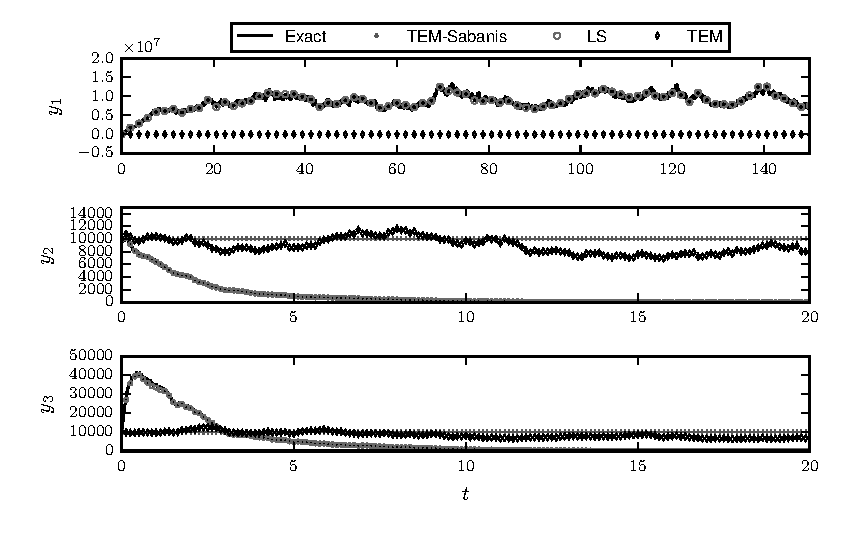
\includegraphics[width=\linewidth]{%
			./IMAGENES/LIPSCHITZ/InternalHIVDynamics.eps}
			}
		\end{overlayarea}
		\column{.4\textwidth}
		\begin{overlayarea}{\textwidth}{.8\textheight}
			\only<2>{
				$\gamma = \num{0.5}$,
				$\eta = \num{0.5}$,
				$\lambda = \num{e6}$, 
				$\delta = \num{0.1}$,
				$\beta = \num{e-8}$,
				$\alpha = \num{0.5}$,
				$N_0= \num{100}$,
				$\mu = \num{5}$,
				$\sigma_1 = \num{0.1}$,
				$\sigma_2 = \num{0.1} $,
				\\
				$y_0 = (
				\num{10000},%{\per\cubic\deci\meter}, 
				\num{10000},%{\per\cubic\deci\meter}, 
				\num{10000}.%{\per\cubic\deci\meter}
			)^T$,
				$h=\num{0.125}$.
				\\
				Exacta: BEM $h=\num{e-5}$
			}
			\begin{bibunit}[apalike]
				\nocite{Dalal2008}
				\only<3->{
					\putbib	
				}
			\end{bibunit}
		\end{overlayarea}
	\end{columns}	
\end{frame}
